%
% Priloha A
%
\chapter{Obsah CD}
Na priloženom CD sa nachádzajú nasledovné súbory a~adresáre:
\begin{itemize}
\item \textbf{doc -} zdrojové súbory tohoto textu v~\LaTeX-ovom formáte 
spolu s~elektronickou verziou vo formáte PDF
\item \textbf{src -} zdrojové súbory plánovača testov spolu s~hlavičkami 
testov používaných v~praxi
\item \textbf{README.txt -} textový súbor obsahujúci príklady spustenia
\end{itemize}



%
% Priloha B
%
\chapter{Ukážka jednoduchého plánu testov z~praxe}
\label{priloha:jednoduchy_plan_testov}
Na nasledujúcej strane je zobrazený plán testov z~produktu MCO,
ktorý pozostáva z~desiatich clusterov. Z~obrázku vyplýva, že pre potreby
týchto clusterov je potrebné spustiť celkovo 19 prerekvizít a~19 
odrekvizít. Pre otestovanie produktu týmito desiatimi clustermi je 
potrebné vykonať ďalších 38 testov, ktoré slúžia na zmenu konfigurácie
systému a~na obnovu týchto zmien. 

Uvedený plán obsahuje celkovo 48 testov a~je relatívne jednoduchý.
V~regresných testoch sa aktuálne používa plán testov, ktorý v~prípade 
produktu MCO pozostáva z~viac ako 3100 testov.
Plán testov každodenne používaný v~regresnom testovní produktu SMSCv5 
pozostáva z~približne 3000 testov.

Príkaz pre naplánovanie a~spustenie regresnej sady každodenne 
používanej v~produkte MCO je zobrazený na obrázku 
\ref{obrazok:priklad_spustania_testov}.

\begin{figure}[h]
  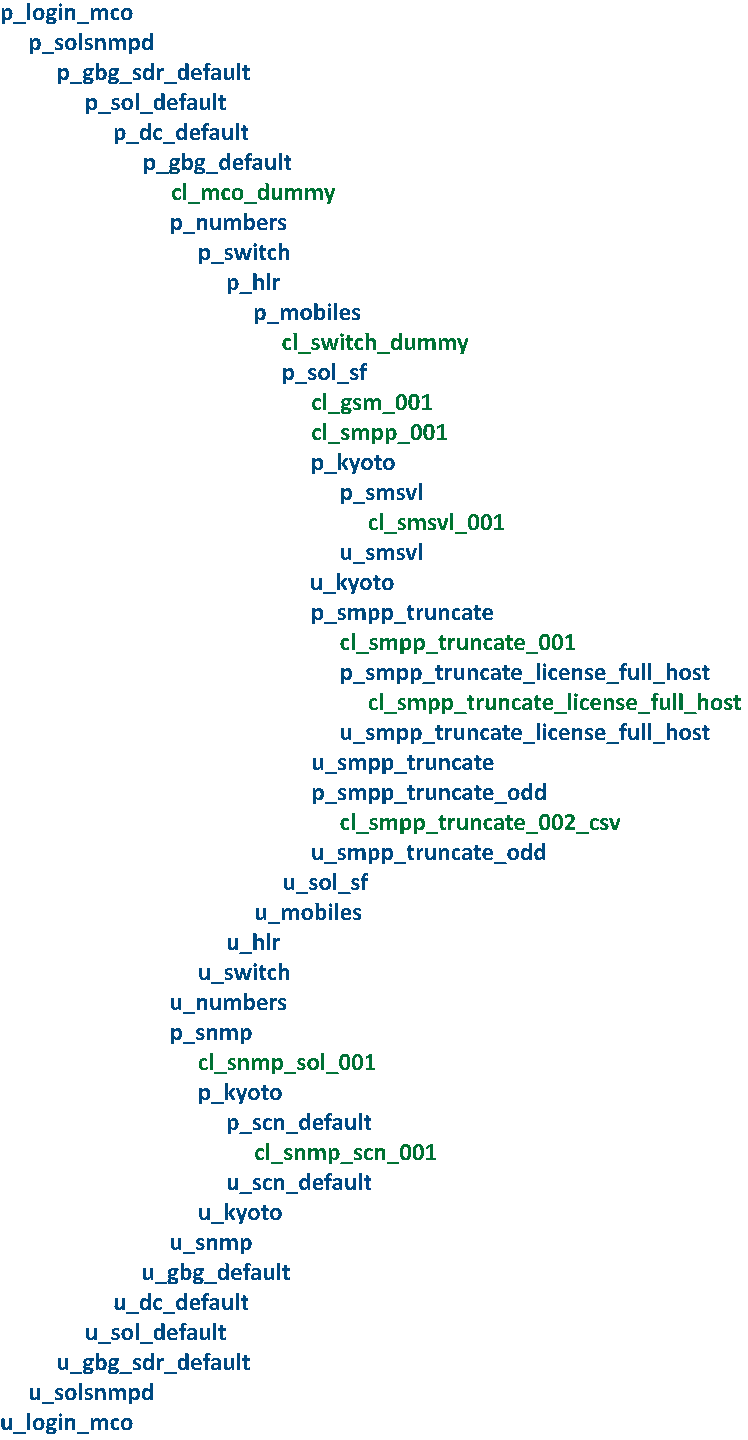
\includegraphics[scale=0.90]{ukazka_jednoducheho_planu}
  \caption{Ukážka jednoduchého plánu testov}
\end{figure}



%
% Priloha C
%
\chapter{Zmeny prevedené do zdrojových súborov a~odovzdané súbory}
\label{priloha:zmeny_do_zdrojakov}
Pri implementovaní rozšírenia plánovaču testov som musel upraviť zdrojové
kódy dvoch hlavných súborov plánovača testov, vytvorených firmou Acision.
Približné zmeny týchto dvoch zdrojových súborov sú nasledovné:

\noindent Zmeny prevedené v~súbore \textbf{Run\_test.tcl}: \\
Riadky: 1426--1430, 1453--1457, 1460--1486 a~ďalej riadky 1488 až 1500.\\
Celkovo približne 50 riadkov kódu (bez komentárov).
\\
\\
\noindent Zmeny prevedené v~súbore \textbf{tstmng.tcl}: \\
Riadky: 115--125, 2245--2253, 2285--2307, 2536--2567, 2607--2609, 
3080--3082, 3184--3187, 3221--3228 a~riadky 3237 až 3245. \\
Ďalej riadky: 2345, 2350, 2354, 2364, 2369, 2395, 2400, 2409, 2442, 
2462, 2467, 2473, 2489, 2513, 2518, 2523, 2528 a~2533. \\
Celkovo približne 123 riadkov kódu (bez komentárov).
\\
\\
Pri odovzdávaní zdrojových súborov som navyše odovzdal len súbory,
potrebné pre beh plánovača testov. Jednotlivé testy pre produkty MCO
a~SMSCv5 boli odstránené a~nahradené jednoduchou funkciou 
\texttt{cl\_wait\_random\_ok} umiestnenou v~súbore \textbf{CL-MY.tcl}. 

Hlavičky testov v~súboroch \textbf{TEST.ALL} a~\textbf{TEST.REVIEW\_23} 
boli ponechané priamo z~produktov MCO a~SMSCv5. V~týchto súboroch som 
však zmenil popis testov (informácia \textit{Description}) 
a~funkcionalitu (informácia \textit{Function}) popísané v~kapitole 
\ref{sekcia:princip_pouziteho_planovaca}.
Jednotlivé závislosti medzi testami ostali ponechané, a~je teda možné 
vytvoriť test plány, ktoré sa používajú priamo v~praxi.
Súbory \textbf{KNOWN.BUGS} ostali ponechané priamo z~týchto dvoch 
produktov bez zmeny. 

Medzi odovzdanými súbormi sa taktiež nachádzajú dva štatistické súbory 
slúžiace napríklad pre výpočet celkovej dĺžky trvania testovania. 
Medzi tieto súbory patrí súbor \textbf{TTT\_stat\_MCO.txt} (pre produkt MCO) 
a~súbor \textbf{TTT\_stat\_SMSC.txt} (pre produkt SMSCv5).
Tieto súboy obsahujú presné informácie o~dĺžkach trvania jednotlivých 
testov v~týchto dvoch produktoch. 
Pre využitie týchto súborov pre konkrétny produkt je potrebné jeden 
z~týchto súborov vložiť do logovacieho adresára \textit{Log/Stat} 
a~premenovať ho na súbor \textbf{TTT\_stat.txt}.
V~prípade použitia týchto štatistických súborov plánovač testov spočíta
odhadovaný čas dĺžky trvania testovania pre každý testovací systém.
Tento čas sa počíta na základe predošlého regresného testovania,
nakoľko sa pri každom testovaní zaznamenávajú časy behu jednotlivých 
testov.



%
% Priloha D
%
\chapter{Ukážka progress baru}
\label{priloha:ukazka_progress_baru}
\begin{figure}[h]
  \begin{center}
    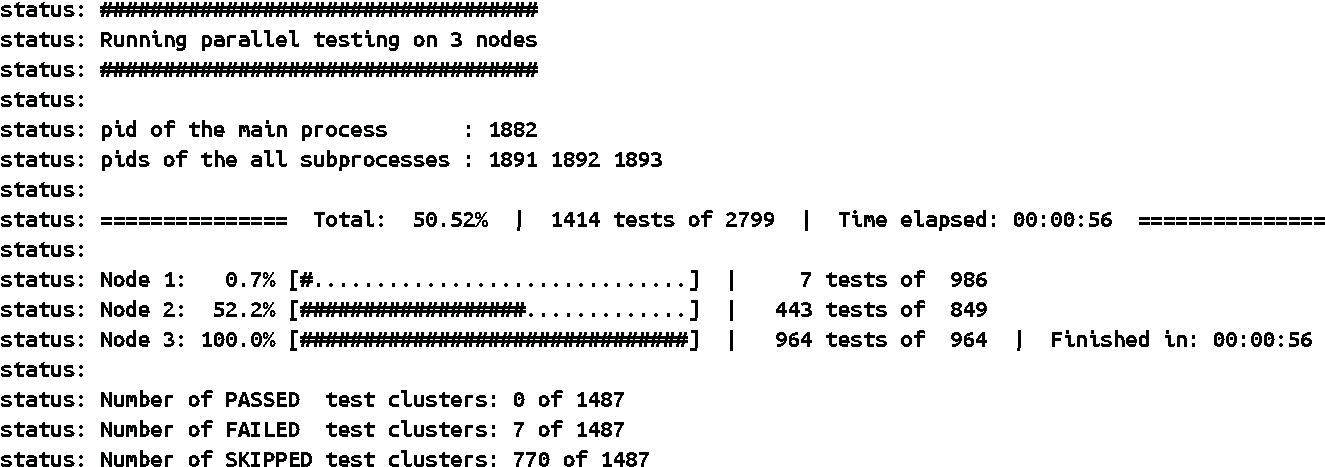
\includegraphics[scale=0.65,angle=90]{ukazka_progress_baru}
    \caption{Ukážka progress baru s~väčšou šírkou terminálu}
  \end{center}
\end{figure}



%
% Priloha E
%
\chapter{Prínos práce pre produkt MCO}
\label{priloha:graf_mco}
Nasledujúci graf zobrazuje závislosť medzi počtom použitých testovacích
systémov a~časom potrebným pre otestovanie produktu MCO regresnou 
sadou testov.

\begin{figure}[h!]
\begin{tikzpicture}[x=1.4cm,y=0.6cm]

  \def\xmin{1}
  \def\xmax{10}
  \def\ymin{0}
  \def\ymax{16}

  % grid
  \draw[style=help lines, ystep=2, xstep=1] (\xmin,\ymin) grid
  (\xmax,\ymax);

  % axes
  \draw[->] (\xmin,\ymin) -- (\xmax,\ymin) node[right] {počet systémov};
  \draw[->] (\xmin,\ymin) -- (\xmin,\ymax) node[above] {čas [h]};

  % xticks and yticks
  \foreach \x in {1,2,...,10}
    \node at (\x, \ymin) [below] {\x};
  \foreach \y in {2,4,...,16}
    \node at (\xmin,\y) [left] {\y};

  \draw[color=blue] plot[smooth,mark=*,mark size=2pt] file {mco.dat}
   node [right] {MCO};

\end{tikzpicture}
\end{figure}



%
% Priloha F
%
\chapter{Prínos práce pre produkt SMSCv5}
\label{priloha:graf_smsc}
Nasledujúci graf zobrazuje závislosť medzi počtom použitých testovacích
systémov a~časom potrebným pre otestovanie produktu SMSCv5 regresnou 
sadou testov.

\begin{figure}[h!]
\begin{tikzpicture}[x=1.4cm,y=0.6cm]

  \def\xmin{1}
  \def\xmax{10}
  \def\ymin{0}
  \def\ymax{16}

  % grid
  \draw[style=help lines, ystep=2, xstep=1] (\xmin,\ymin) grid
  (\xmax,\ymax);

  % axes
  \draw[->] (\xmin,\ymin) -- (\xmax,\ymin) node[right] {počet systémov};
  \draw[->] (\xmin,\ymin) -- (\xmin,\ymax) node[above] {čas [h]};

  % xticks and yticks
  \foreach \x in {1,2,...,10}
    \node at (\x, \ymin) [below] {\x};
  \foreach \y in {2,4,...,16}
    \node at (\xmin,\y) [left] {\y};

  \draw[color=blue] plot[smooth,mark=*,mark size=2pt] file {smsc.dat}
   node [right] {SMSCv5};

\end{tikzpicture}
\end{figure}
